\documentclass[a4paper,12pt]{book}
\usepackage[utf8x]{inputenc}
\usepackage[spanish]{babel}
\usepackage{amsmath, amsthm, amsfonts}
\usepackage{graphicx}
\usepackage{pstricks} % para color
\usepackage{pst-node} % para diagramas
\usepackage{pst-plot} % para representacion de datos
		      % funciones, etc
\usepackage{pst-text}
\usepackage{pst-coil}
\usepackage{hyperref}
\usepackage{color}
\usepackage{fancyhdr}
\usepackage{eso-pic,calc}                        
\usepackage{multicol}

\usepackage{listings}
% Utilidades
%--------------------------------------------------------------------------
\newtheorem{thm}{Teorema}[section]
\newtheorem{cor}[thm]{Corolario}
\newtheorem{lem}[thm]{Lema}
\newtheorem{prop}[thm]{Proposición}
\theoremstyle{definition}
\newtheorem{defn}[thm]{Definición}
\theoremstyle{remark}
\newtheorem{rem}[thm]{Observación}

\pdfpagewidth 6in
\pdfpageheight 9in
\setlength\topmargin{0in}
\setlength\headheight{0in}
\setlength\headsep{0in}
\setlength\textheight{7.7in}
\setlength\textwidth{6.5in}
\setlength\oddsidemargin{0in}
\setlength\evensidemargin{0in}
\setlength\headheight{25pt}
\setlength\headsep{0.25in}

%opening
\pagestyle{plain}
%opening
\frontmatter
\makeindex
\begin{document}
\begin{figure}[hc]
\begin{titlepage}
\begin{center}
{\Large \textbf{Ingenier\'ia T\'ecnica en Inform\'atica de Gesti\'on\\Laboratorio de Programaci\'on Avanzada}}
\end{center}
\end{titlepage}
\end{figure}
\begin{figure}[hc]
\begin{center}
{\Large \textbf{Curso 2010/2011\\Pr\'actica Funcional N: 5}}
\end{center}
\end{figure}
\begin{figure}[hc]
\begin{center}
{\large \textbf{Autor: 09047323C - Lucena Pumar, Diego Antonio}}
\end{center}
\end{figure}
\newpage
Reservados algunos derechos de autor amparados en la Ley internacional del
Copyright.


\textcopyright\ Diego Antonio Lucena Pumar.



Puedes libremente distribuir este documento, y usarlo para tus propios
cometidos, pero nunca ser\'an el de lucro.



En la Villa de Meco a 24 de Agosto de 2011.


Fecha de \'ultima revisi\'on: Meco, 24 de Agosto de 2011.


Editor: Diego Antonio Lucena Pumar.


Maquetado directamente en \LaTeXe


\newpage
\begin{figure}[hc]
\begin{flushright}
\textit{\textit{BLA, BLA...}}
\end{flushright}
\end{figure}
\newpage{\pagestyle{empty}\cleardoublepage}
\begin{figure}[c]
\begin{flushright}
\textit{``BLA, BLA, BLA...''}
\end{flushright}
\begin{flushright}
\textbf{BLA...}
\end{flushright}
\end{figure}

%\newpage{\pagestyle{empty}\cleardoublepage}
% \chapter{Pr\'ologo}
He aqu\'i que como nota concluimos. Teor\'ia de Sistemas Operativos Distribuidos
es un libro de texto que como bien su nombre advierte honda y gira en torno a
los fundamentos de estos ``aut\'omatas''. El texto se presenta conciso, se ha
hecho especial incapie en las definiciones, fundamentales para el entendimiento
de la materia. As\'i mismo, se ha utilizado cierta notaci\'on con el objeto de
clarificar mediante s\'imbolos aquello que encierra un significado indivisible.


El texto comienza fundamentando el proceso distribuido. Se trata su
comunicaci\'on y planificaci\'on. Seguido se dan ejemplos de m\'aquinas que
trabajan con este tipo de unidades de datos. 


La segunda parte aborda la gesti\'on de la memoria, tema delicado y principal
para entender que es realmente un sistema distribuido. Por \'ultimo son
analizados los sistemas de ficheros y tres casos implementados: \textit{MS-DOS}
(aun no siendo puramente distribuido), \textit{NFTS} y el sistema de ficheros de
UNIX SYSTEM V, \textit{UFS}.


Espero que el trabajo vertido en est\'a obra sea de su agrado.


Reciba un cordial saludo. Diego Antonio Lucena Pumar.
% \newpage{\pagestyle{empty}\cleardoublepage}
% \chapter{Fe de Erratas}
Como autor y editor de este libro quiero invitarle a que con sus inter\'eses y
apreciaciones hagamos de este un texto mucho m\'as preciso. Por ello, es
indudable, dado la cantidad de tareas que he realizado para confeccionar el
presente, que en alguno de los pasos haya cometido alg\'un tipo de error sin
intencionar. Si lo ha detectado y tiene tiempo, puede escribirme a: diego.lucena.pumar@gmail.com 


Gracias de antemano.
% \newpage{\pagestyle{empty}\cleardoublepage}
\tableofcontents
\newpage{\pagestyle{empty}\cleardoublepage}
\mainmatter
\pagestyle{fancy}
% \addcontentsline{toc}{chapter}{Tabla de notaci\'on}
% \chapter*{Tabla de notaci\'on} 
La misma describe la notaci\'on usada a los largo del texto repecto de los elementos que se tratan con un plano algebraico.
\begin{table}[h]
\begin{center}
\begin{tabular}{|c|l|}
\hline
\textit{S\'imbolo} & \textit{Significado}\\ \hline 
\hline 
$\varsigma$ & Usuario \\ \hline
$\chi$ & Proceso \\ \hline
$\rho$ & M\'aquina \\ \hline
$\upsilon$ & Recurso \\ \hline
$\sigma$ & P\'agina de memoria \\ \hline
$n$ & N\'umero variable de elementos \\ \hline
$t$ & Tiempo variable \\ \hline
\end{tabular} 
\caption{Tabla de s\'imbolos.}
\end{center}
\end{table}

% \newpage{\pagestyle{empty}\cleardoublepage}
\chapter{Planteamiento del problema}

\paragraph{Nota:} Presentación basada em el texto: \cite{aalpa}.

\section{Condiciones}

La presente prática gira en torno a la creación de una aplicación en base al
lenguaje de programación funcional ``Caml'' en su versión ligera. Dicha
aplicación ha de ser un juego ``Sudoku Dodeka'', versión de popular juego de
cifras ``Sudoku''. Las reglas de este variante se detallan a continuación:

\begin{itemize}
\item Las posibles fichas del juego contiene las cifras decimales de: 0 a 9 y
las teras A y B.
\item Para todos los elementos de una misma fila no se han de repetir dos fichas
iguales.
\item Para todos los elementos de una misma columna no se han de repetir dos
fichas iguales.
\item Para todos los elementos de una mismo ret\'angulo (3x4) no se han de
repetir dos fichas iguales. 
\item El juego termina cuando se cumplen las reglas anteriormenete expuestas y
no hay ninguna casilla en blanco ('.').
\end{itemize}

\section{Funciones propuestas}

Para el mismo juego se proponen una funciones básicas que deben ser parte del
código. Las misma son:

\begin{itemize}
\item formarSudoku: Toma como argunmento una lista de carácteres (tablero) y
devuelve el Sudoku formateado.
\item mostrar tablero: Recibe un tablero como argumento y devuelve el dibujo del
mismo.
\item elemento casilla tablero: Devuelve el valor que tiene asignado dicha
casilla en el tablero.
\item posibles casilla tablero: Devuelve una lista con los valores que puede
tomar dicha casilla en el tablero.
\item resuelto tablero: Devuelve cierto si el Sudoku está resuelto y falso en
caso contrario.
\end{itemize}

\section{Tipos de Sudoku}

Existe tres tipos de Sudoku planteados:

\begin{itemize}
\item Sudoku fácil: Se trata de un Sudoku sencillo en el que su solución viene
dada por eliminación de posibles valores sobre las distintas casillas.
\item Sudoku difícil: Se trata de un Sudoku en el que la única forma de obtener
su solución se hace con algorítmia compleja (técnica de BackTraking)
\item Sudoku imposible: Se trata de un Sudoku en el que por la disposición de
las fichas en el tablero es imposible llegar a una solución.
\end{itemize}





\newpage{\pagestyle{empty}\cleardoublepage}
\chapter{Manual de Usuario}

\section{Cuadro de Mando General (CMG)}

\textit{Diego's Software \& Systems} se complace en presentarle el simulador de una
Ciudad Deportiva. A grandes rasgos podr\'a observar un comportamiento aleatorio
en cada simulaci\'on con distintas opciones que da a la aplicaci\'on en si, gran
versatilidad y realismo para probar este tipo de entornos.

\begin{figure}[h]
\begin{center}
 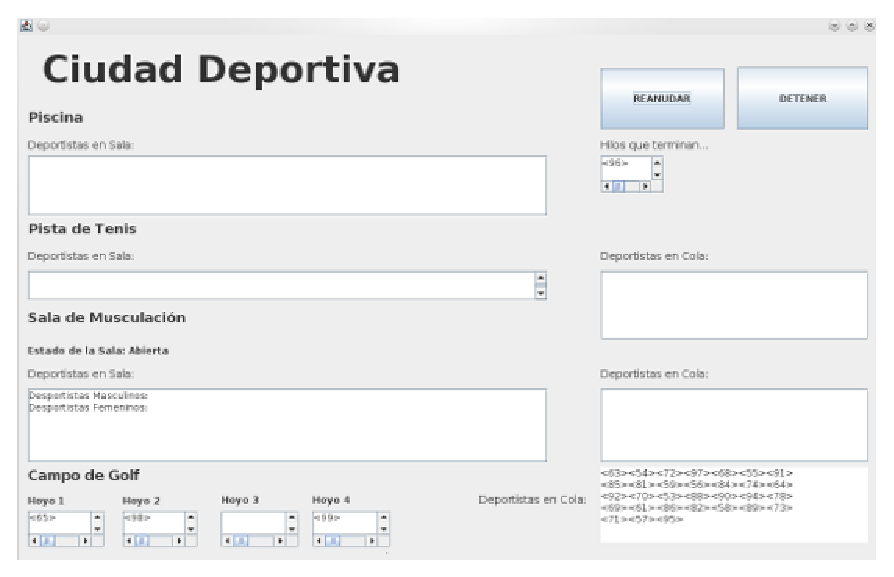
\includegraphics{./images/generalCiudadDeportiva.eps}
 % generalCiudadDeportiva.eps: 0x0 pixel, 300dpi, 0.00x0.00 cm, bb=
\end{center}
\caption{Cuadro de Mando General (CMG).}
\end{figure}


El Cuadro de Mando General se muestra en la Figura 2.1. Diremos que tiene como
funci\'on principal el proporcionar un total control de la ejecuci\'on del
programa. Podr\'a observar d\'onde se encuentra cada doportista y como cumple
sus objetivos, desde que acude a la Piscina hasta que finaliza su ciclo. 

\begin{figure}[h]
\begin{center}
 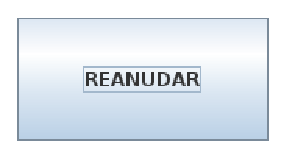
\includegraphics{./images/botonReanudar.eps}
 % botonReanudar.eps: 0x0 pixel, 300dpi, 0.00x0.00 cm, bb=
\end{center}
\caption{Vista detallada del bot\'on Reanudar del CMG.}
\end{figure}


\begin{figure}[h]
\begin{center}
 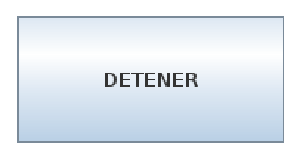
\includegraphics{./images/botonDetener.eps}
 % botonDetener.eps: 0x0 pixel, 300dpi, 0.00x0.00 cm, bb=
\end{center}
\caption{Vista detallada del bot\'on Detener del CMG.}
\end{figure}


\begin{figure}[h]
\begin{center}
 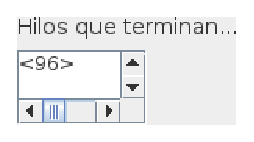
\includegraphics{./images/findeHilos.eps}
 % findeHilos.eps: 0x0 pixel, 300dpi, 0.00x0.00 cm, bb=
\end{center}
\caption{Vista detallada la finalizaci\'on de la actividad de un deportista.}
\end{figure}








\newpage{\pagestyle{empty}\cleardoublepage}
\chapter{Pruebas}






\newpage{\pagestyle{empty}\cleardoublepage}
\addcontentsline{toc}{chapter}{\bibname}
%\onecolumn
%\let\OLDthebibliography=\thebibliography
%\def\thebibliography#1{\OLDthebibliography{#1}
%    \addcontentsline{toc}{chapter}{\bibname}}
\bibliography{lib.bib}\bibliographystyle{alpha}
% \newpage{\pagestyle{empty}\cleardoublepage}
% \addcontentsline{toc}{chapter}{\'Indice alfab\'etico}
% \printindex
\end{document} 